\chapter{Алгоритмы работы с пользователем}

    В данном разделе будут представлены алгоритмы работы с потенциальным пользователем %
    веб-приложения.

    \section{Диаграммы активности}
        Диаграмма активности  “Регистрация пациента”\ представляет %
        собой последовательность следующих действий:
        \begin{enumerate}
            \item Пользователь отправляет данные для регистрации;
            \item Происходит проверка введенных данных, в случае если были предоставлены %
            некоректные данные, пользователь вводит данные снова, а в %
            случае успешной проверки - происходит следующая этап взаимодейсвия;
            \item Происходит проверка на уникальность пациента, в %
            случае не уникальности пациента - пользователь вводит данные %
            снова, в ином случае - происходит регистрация пользователя;
        \end{enumerate}

        Диаграмма активности “Регистрация пациента” изобрaжена на рисунке \ref{diagram-registration}.
        \begin{figure}[H]%current location
            \centering
            \scalebox{0.42}{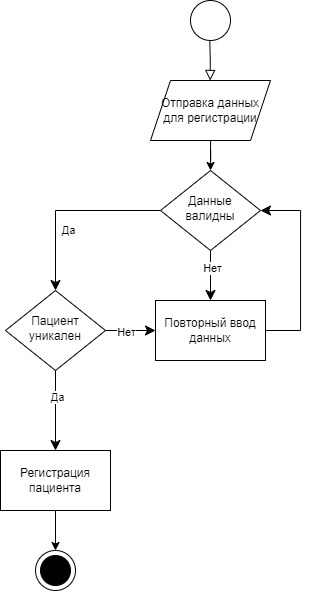
\includegraphics{pics/diagrams/register.png}}
            \caption{Диаграмма активности “Регистрация пациента”.} \label{diagram-registration}
        \end{figure} 

        Диаграмма активности  “Получить список пациентов” представляет собой %
        последовательность следующих действий:

        \begin{enumerate}
            \item Пользователь отправляет запрос на получение списка пациентов;
            \item Происходит проверка на существование данных, в случае %
            существовании данных происходит следующий этап - получение списка %
            пациентов, в ином случае - происходит извещение доктора об отсутствии пациентов;
        \end{enumerate}
        
        Диаграмма активности  “Получить список пациентов” изобрaжена на рисунке \ref{diagram-patient-list}.

        \begin{figure}[H]%current location
            \centering
            \scalebox{0.6}{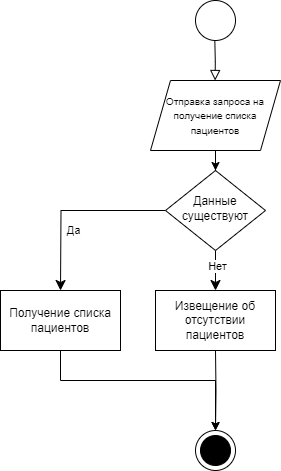
\includegraphics{pics/diagrams/patient-list.png}}
            \caption{Диаграмма активности  “Получить список пациентов”.} \label{diagram-patient-list}
        \end{figure} 

        Диаграмма активности “Администрирование данных о врачах” %
        представляет собой последовательность следующих действий:
        \begin{enumerate}
            \item Менеджер отправляет запрос на получение данных о врачах;
            \item Происходит проверка корректности данных, если данные %
            корректны, то происходит следующий этап, в ином случае происходит %
            отказ в доступе к пациентам для врача;
            \item Происходит проверка отзывов лечащего врача, %
            оставленных пациентами, в случае, если отзывы приемлемы врач %
            утверждается, в ином случае - происходит отказ в доступе к пациентам %
            для врача;
        \end{enumerate}
        
        Диаграмма активности “Администрирование данных о врачах” изображена %
        на рисунке \ref{diagram-doctor-admin}.
        \begin{figure}[H]%current location
            \centering
            \scalebox{0.6}{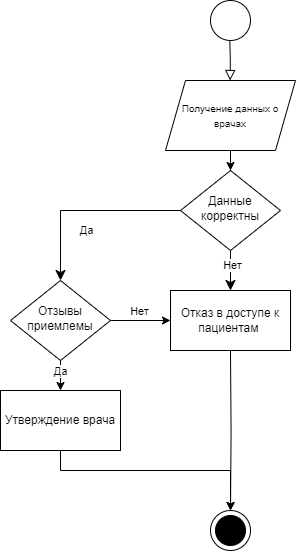
\includegraphics{pics/diagrams/doctor-admin.png}}
            \caption{Диаграмма активности “Администрирование данных о врачах”.} \label{diagram-doctor-admin}
        \end{figure} 
    
    \section{Контекстные диаграммы взаимодейсвия}
        В данном подразделе представлена модель в нотации IDEF3, которая %
        описывает информационные потоки и взаимоотношения между процессами %
        обработки информации и объектами, являющимися частью этих процессов. %
        Модель представлена в виде контекстной диаграммы (рисунок \ref{context-diagram}), которая %
        представляет собой графическое представление основных компонентов системы и %
        их взаимосвязей и позволяет определить основные процессы и объекты, которые %
        участвуют в обработке информации, а также информационные потоки между ними. %
        
        \begin{figure}[H]%current location
            \centering
            \scalebox{0.6}{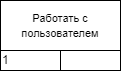
\includegraphics{pics/IDEF3/context-diagram.png}}
            \caption{Контекстная диаграмма (IDEF3)} \label{context-diagram}
        \end{figure} 
        
        Декомпозиции этой диаграммы изобажена на рисунке \ref{context-decomposition}. %
        Декомпозиция представляет собой более детальное %
        представление процессов и объектов, описанных в контекстной диаграмме, позволяет %
        более подробно описать каждый процесс и объект, а также их взаимосвязи. Кроме того, %
        она включает в себя описание входных и выходных данных, используемых ресурсов и %
        исполнителей, необходимых для выполнения процессов.


        \begin{landscape}
            \begin{figure}[H]%current location
                \centering
                \scalebox{0.4}{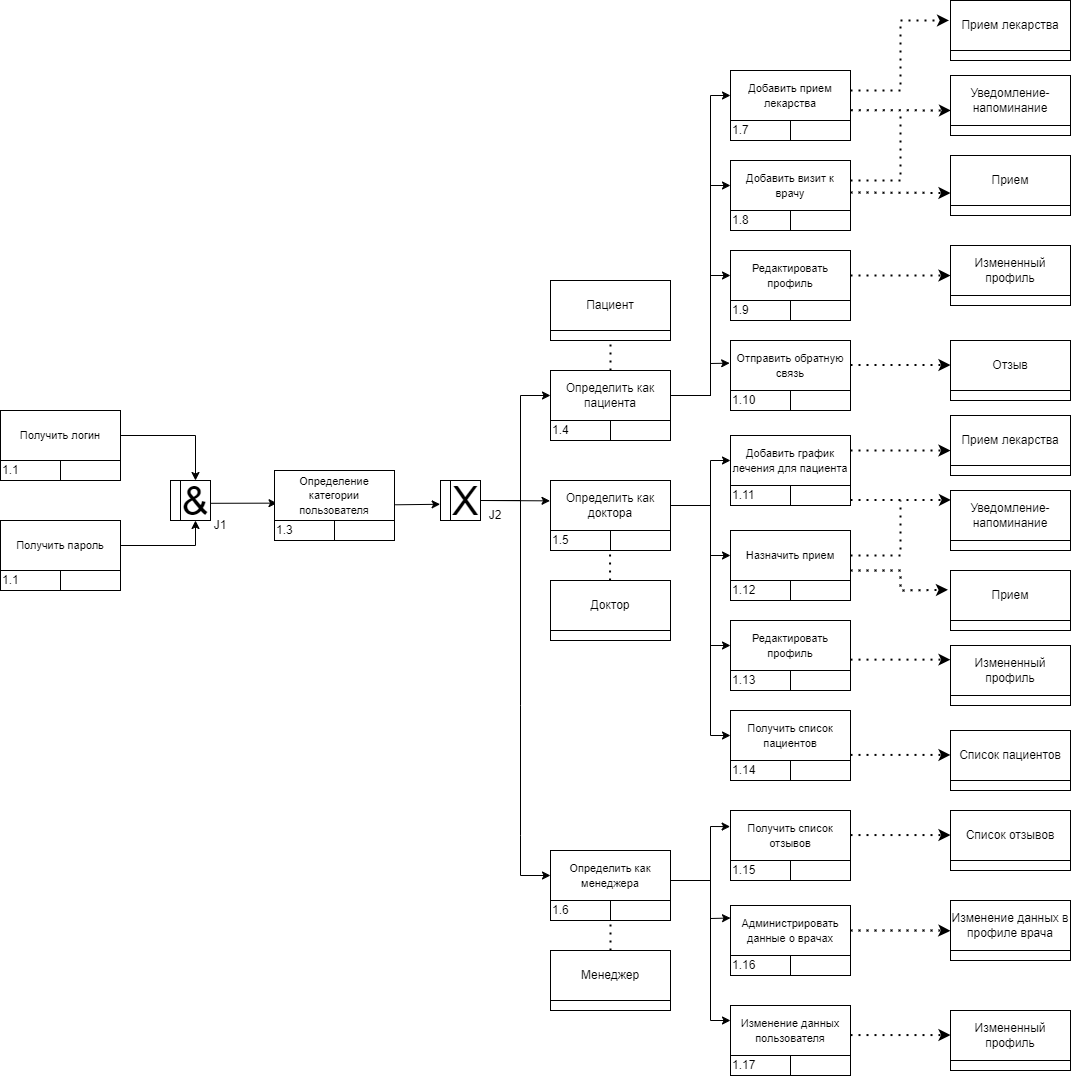
\includegraphics{pics/IDEF3/context-decomposition.png}}
                \caption{Декомпозиция контекстной диаграммы} \label{context-decomposition}
            \end{figure} 
        \end{landscape}

        Декомпозиции блока “Администрировать данные о врачах” представлена на рисунке \ref{context-doctor-admin}

        \begin{figure}[H]%current location
            \centering
            \scalebox{0.5}{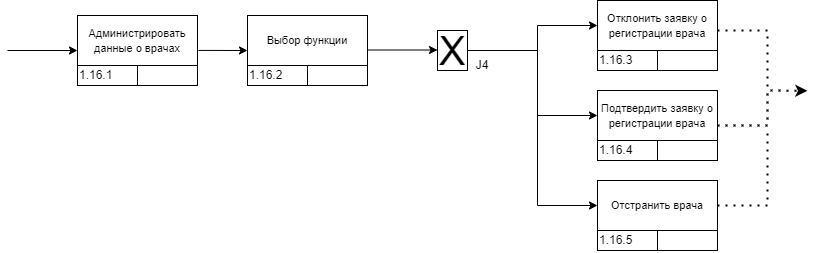
\includegraphics{pics/IDEF3/context-doctor-admin.png}}
            \caption{Декомпозиции блока “Администрировать данные о врачах”} \label{context-doctor-admin}
        \end{figure} 

        Декомпозиция блока Декомпозиция блока “Получить список пациентов” представлена на рисунке \ref{context-patient-list}

        \begin{figure}[H]%current location
            \centering
            \scalebox{0.5}{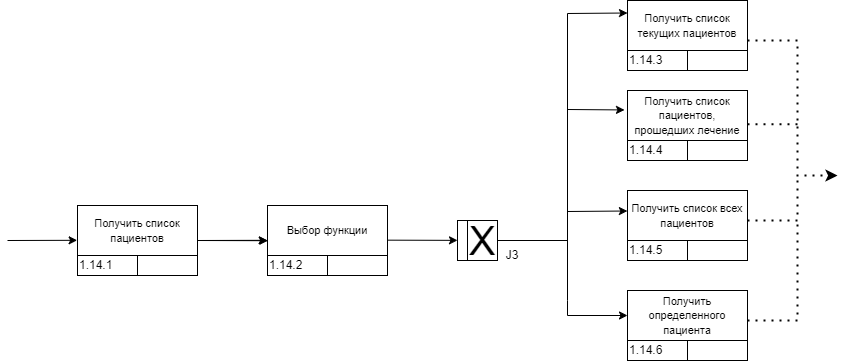
\includegraphics{pics/IDEF3/context-user-list.png}}
            \caption{Декомпозиции блока “Администрировать данные о врачах”} \label{context-patient-list}
        \end{figure} 
        
        Декомпозиция блока “Редактировать профиль” представлена на рисунке \ref{context-change-profile}

        \begin{figure}[H]%current location
            \centering
            \scalebox{0.5}{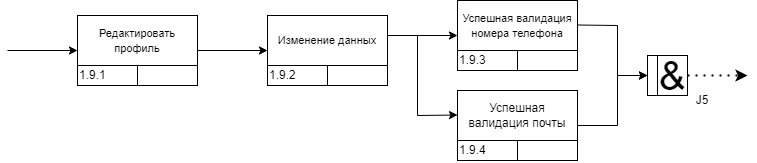
\includegraphics{pics/IDEF3/context-change-profile.png}}
            \caption{Декомпозиции блока “Администрировать данные о врачах”} \label{context-change-profile}
        \end{figure} 